%Przykładowy plik ułatwiający złożenie projektu dyplomowego inżynierskiego.
%UWAGA: Generowany napis na stronie tytułowej o treści PROJEKT DYPLOMOWY INŻYNIERSKI został zaproponowany przeze mnie i nie jest, póki co, potwierdzony przez władze wydziału. Przed ostatecznym oddaniem tak złożonej pracy należy upewnić się jaka powinna być treść tego napisu. W momencie gdy uzyskam informację na temat treści tego napisu, dokonam niezbędnych zmian w źródłach.
\documentclass[printmode]{mgr}
%opcje klasy dokumentu mgr.cls zostały opisane w dołączonej instrukcji

%poniżej deklaracje użycia pakietów, usunąć to co jest niepotrzebne
%\usepackage{polski} %przydatne podczas składania dokumentów w j. polskim
\usepackage[polish]{babel}%alternatywnie do pakietu polski, wybrać jeden z nich
%\usepackage[OT4,plmath]{polski}
\usepackage[utf8]{inputenc} %kodowanie znaków, zależne od systemu
\usepackage[T1]{fontenc} %poprawne składanie polskich czcionek

%pakiety do grafiki
\usepackage{subfigure}
\usepackage{listings}
\usepackage{graphicx}
\usepackage{epstopdf}
\usepackage{subfigure}
\usepackage{psfrag}

\lstset{ %
language=C++,                	% choose the language of the code
basicstyle=\scriptsize,       		% the size of the fonts that are used for the code
numbers=left,                   % where to put the line-numbers
numberstyle=\footnotesize,      % the size of the fonts that are used for the line-numbers
stepnumber=2,                   % the step between two line-numbers. If it's 1 each line 
                                % will be numbered
numbersep=5pt,                  % how far the line-numbers are from the code
showspaces=false,               % show spaces adding particular underscores
showstringspaces=false,         % underline spaces within strings
showtabs=false,                 % show tabs within strings adding particular underscores
frame=single,	                % adds a frame around the code
tabsize=2,	                % sets default tabsize to 2 spaces
captionpos=b,                   % sets the caption-position to bottom
breaklines=true,                % sets automatic line breaking
breakatwhitespace=false,        % sets if automatic breaks should only happen at whitespace
title=\lstname,                 % show the filename of files included with \lstinputlisting;
                                % also try caption instead of title
escapeinside={\%*}{*)},         % if you want to add a comment within your code
morekeywords={*,...}            % if you want to add more keywords to the set
}

%pakiety dodające dużo dodatkowych poleceń matematycznych
\usepackage{amsmath}
\usepackage{amsfonts}

%pakiety wspomagające i poprawiające składanie tabel
\usepackage{supertabular}
\usepackage{array}
\usepackage{tabularx}
\usepackage{hhline}

%pakiet wypisujący na marginesie etykiety równań i rysunków zdefiniowanych przez \label{}, chcąc wygenerować finalną wersję dokumentu wystarczy usunąć poniższą linię
%\usepackage{showlabels}

%definicje własnych poleceń
\newcommand{\R}{I\!\!R} %symbol liczb rzeczywistych, działa tylko w trybie matematycznym
\newtheorem{theorem}{Twierdzenie}[section] %nowe otoczenie do składania twierdzeń

%dane do złożenia strony tytułowej
\title{Podatny manipulator planarny - budowa i sterowanie}
\engtitle{Vulnerable planar manipulator - design and control}
\author{Michał Kot}
\supervisor{dr inż. Janusz Jakubiak, I-6}
%\guardian{dr hab. inż. Imię Nazwisko Prof. PWr, I-6} %nie używać jeśli opiekun jest tą samą osobą co prowadzący pracę

%\date{2008} %standardowo u dołu strony tytułowej umieszczany jest bieżący rok, to polecenie pozwala wstawić dowolny rok

%poniżej jest lista kierunków i specjalności na wydziale elektroniki, należy wybrać właściwe lub dopisać jeśli nie ma odpowiednich
\field{Automatyka i Robotyka (AIR)}
\specialisation{Robotyka (ARR)}

%tutaj zaczyna się właściwa treść dokumentu
\begin{document}
\bibliographystyle{plabbrv} %tylko gdy używamy BibTeXa, ustawia polski styl bibliografii

\maketitle %polecenie generujące stronę tytułową
\tableofcontents %spis treści

%poniżej znajduje się przykładowa treść dalszej części dokumentu, zainteresowanych zachęcam do rozszyfrowania frazy "Lorem ipsum" :)

\chapter{Wstęp}
Oby gdzieś był

\chapter{Cele projektu} \label{ch:cele}
Celem projektu zrealizowanego w ramach niniejszej pracy magisterskiej jest zaprojektowanie i skonstruowanie planarnego, równoległego
i redundantnego manipulatora, który będzie w stanie analizować siły działające na niego z zewnątrz. Umożliwi to 
zręczne poruszanie się robota w środowisku, ponieważ każda napotkana przeszkoda spowoduje zatrzymanie go bądź też zmusi
do osiągnięcia zadanego położenia w innej konfiguracji przegubów. Dodatkową cechą, która zostanie zaimplementowana w manipulatorze
jest możliwość uczenia się ruchów zadanych manualnie przez operatora -- konkretna ścieżka może zostać zapisana na podstawie
odczytów sił działających na napędy. 

\section{Aspekt inżynierski}
Aspekt inżynierski projektu zakłada zaprojektowanie mechaniki i układu sterowania manipulatora. Jest on ściśle powiązany
z aspektem badawczym (\ref{sec:aspekt_badawczy}), ponieważ dobór parametrów układu mechanicznego musiał zostać poprzedzony
szeregiem analiz i symulacji. Trójwymiarowy model obiektu został wykonany z wykorzystaniem środowiska \texttt{Autodesk Inventor} \cite{autodesk},
które to umożliwia szybkie i wygodnie modelowanie złożonych konstrukcji mechanicznych. Co więcej, posiada on plugin
\texttt{SimMechanics Link} \cite{simmechanics_link}, umożliwiający eksport modelu do toolboxa \texttt{Simulink} środowiska 
\texttt{Matlab} \cite{mathworks}, które jest jednym z najpopularniejszych i najbardziej rozbudowanych aplikacji symulacyjnych.
W trakcie prac z wykorzystaniem Inventora skonstruowane zostały cztery podobne modele manipulatora, które ewoluowały 
w kierunku wersji docelowej. 

Projektowanie i implementacja algorytmów sterowania ..................... bla bla ........................

\section{Aspekt badawczy}\label{sec:aspekt_badawczy}
Opracowanie kryteriów doboru parametrów kinematycznych manipulatora stanowiło jeden z kluczowych elementów aspektu badawczego projektu.
Proporcje długości ramion robota mają istotny wpływ na jakość i wielofunkcyjność jego pracy, w związku z czym definiuje się cały
szereg kryteriów \cite{miary_jakosci}, które różnią się pomiędzy sobą zarówno podejściem, jak i stopniem skomplikowania:
\begin{itemize}
\item ekscentryczność manipulatora, mierząca odległość położenia przegubów od ich pozycji środkowych,
\item manipulowalność manipulatora, która jest miarą wrażliwości efektora na lokalne wariacje konfiguracji,
\item współczynnik uwarunkowania, będący miarą stopnia anizotropowości konfiguracji,
\item dystorsja kinematyczna, jako miara niesztywności kinematyki,
\item objętość przestrzeni roboczej,
\item gęstość objętości kinematyki.
\end{itemize}
W teorii robotyki stosuje się także kombinacje kilku różnych kryteriów. W przypadku niniejszego projektu zastosowane zostało
kryterium mówiące o objętości przestrzeni roboczej, co w przypadku manipulatorów planarnych sprowadza się do powierzchni przestrzeni roboczej. 
Obliczenie przestrzeni z dużą dokładnością dla wielu różnych konfiguracji robota jest niemożliwe bez wykorzystania komputera. W związku
z tym konieczne okazało się napisanie programu z wykorzystaniem języka C++, który wyszukuje optymalną konfigurację parametrów manipulatora. 
Szerzej zostało to opisane w rozdziale \ref{sec:wyznaczenie_wymiarow_manipulatora}.

Istotną częścią aspektu badawczego projektu były także badania porównawcze algorytmów sterowania oraz ocena ich własności.
..................... bla bla ........................


\section{Kinematyka}
Efektorem (chwytakiem) nazywa się zakończenie konstrukcji manipulatora, które często posiada możliwość wymiany bądź modyfikacji. 
Dzięki temu jeden robot może sekwencyjnie wykonywać kilka różniących się od siebie operacji. Przekształcenie geometryczne,
które pozwala wyznaczyć położenie efektora w przestrzeni roboczej na podstawie położeń przegubów manipulatora określa się mianem kinematyki. 
Ze względu na planarność konstruowanego manipulatora wyznaczenie kinematyki sprowadza się do obliczenia położeń X i Y, gdyż
ruch robota odbywa się na płaszczyźnie i współrzędna Z jest stała.





\chapter{Pierwowzór} \label{ch:pierwowzor}
Pomysł na stworzenie planarnego manipulatora zrodził się po przeczytaniu artykułu naukowego
"Hybrid position/force control of a flexible parallel manipulator" \cite{wzor}. 
Autorzy tego artykułu podjęli się stworzenia równoległego manipulatora, którego cechą charakterystyczną
jest elastyczna końcówka umożliwiająca pomiary sił/momentów działających na efektor. 
Jak widzimy na rysunku \ref{rys:pierwowzor_zdjecie}, do pomiaru siły został wykorzystany czujnik sił/momentów
o sześciu stopniach swobody, dzięki czemu możliwe jest wykrycie każdego rodzaju deformacji elastycznej
końcówki. Zaletą takiego rozwiązania jest zdolność do analizy sił i momentów, którymi otoczenie
oddziałuje na efektor. W rezultacie, poprzez zastosowanie hybrydowego sterowania, polegającego
na jednoczesnym kontrolowaniu położenia efektora i sił na niego oddziałujących, jesteśmy w stanie zapewnić
dokładniejszą i bezpieczniejszą interakcję manipulatora z otoczeniem. Wynika to z braku dużych sił powstających
przy wykorzystaniu jedynie kontroli położenia.
\begin{figure}[tp]
\centering
  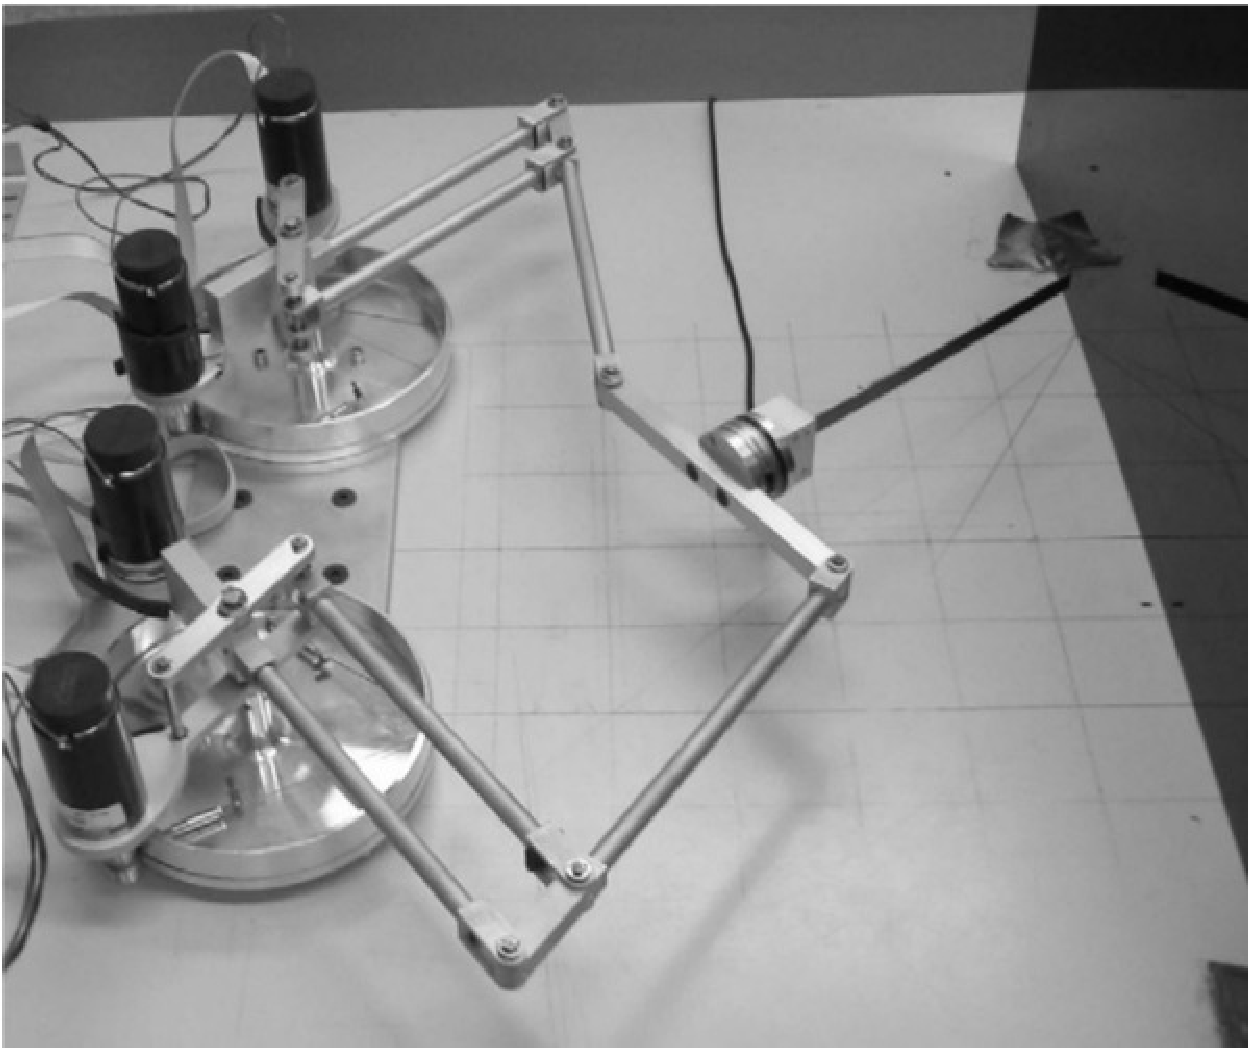
\includegraphics[width=0.6\textwidth]{grafika/pierwowzor_zdjecie}
  \caption{Pierwowzór konstruowanego manipulatora}
  \label{rys:pierwowzor_zdjecie}  
\end{figure}

\section{Różnice w stosunku do pierwowzoru}
Stworzony w ramach niniejszej pracy magisterskiej manipulator różni się jednakże w wielu aspektach od
swojego pierwowzoru. Na rysunku \ref{rys:pierwowzor_model} znajduje się model pierwowzoru, jednakże po szeregu badań i analiz 
okazało się, że konstrukcja tamtego manipulatora nie zakładała redundancji, która jest jednym z
fundamentów tego projektu. Redundancja, która umożliwia osiągnięcie jednego położenia efektora przy pomocy
wielu różnych konfiguracji manipulatora, została zapewniona poprzez wprowadzenie jednego dodatkowego przegubu
pasywnego. Co więcej, w stosunku do pierwowzoru elastyczne ramie połączone z czujnikiem sił i momentów
zostało zastąpione przez inny mechanizm, opisany dokładniej w rozdziale \ref{sec:czujniki_sily}.
Dzięki zmianom w konstrukcji manipulator stworzony w ramach tego projektu posiada większą gamę
potencjalnych zastosowań, np. możliwość uczenia się. 

\begin{figure}[tp]
\centering
  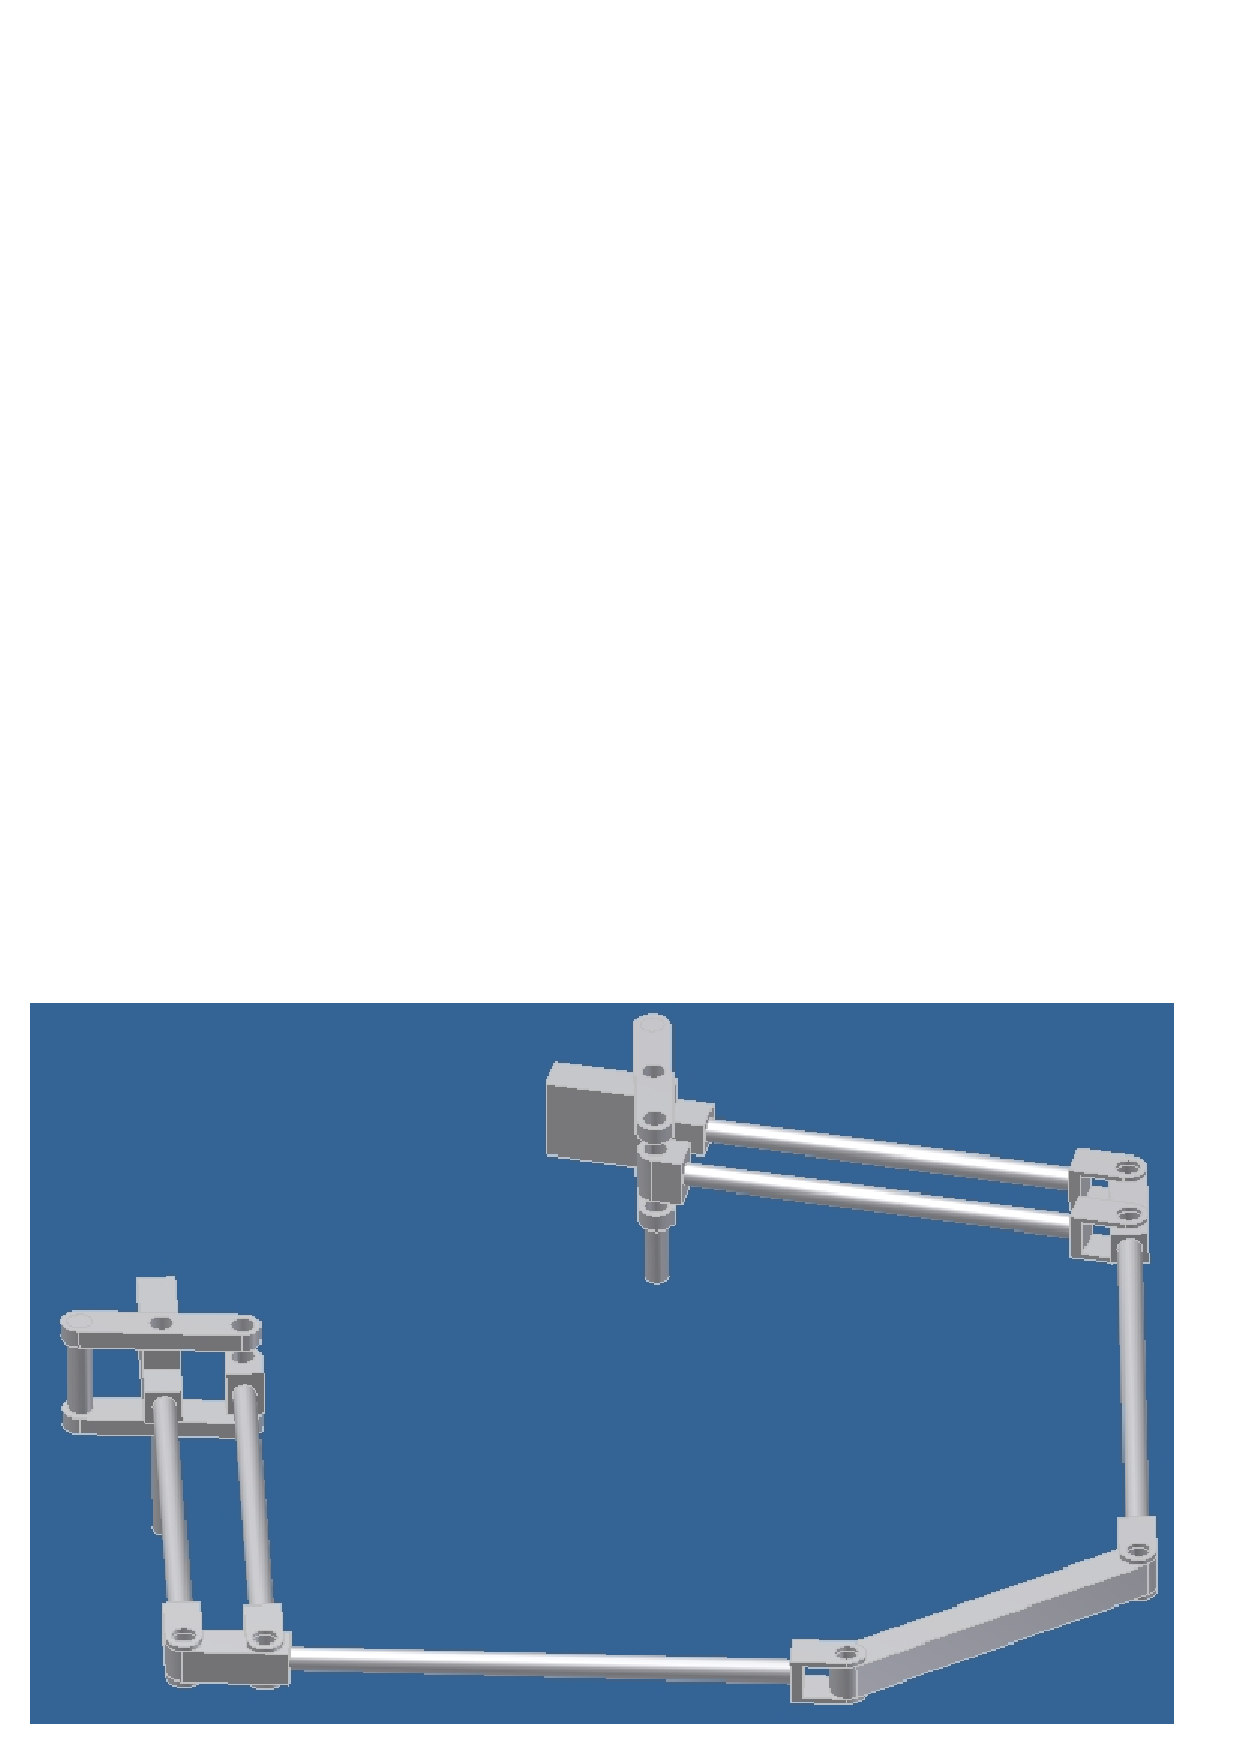
\includegraphics[width=0.6\textwidth]{grafika/pierwowzor_model}
  \caption{Model pierwowzoru konstruowanego manipulatora}
  \label{rys:pierwowzor_model}  
\end{figure}


\section{Inne projekty wykorzystujące podobne rozwiązania}


\chapter{Testowe modele manipulatora}

\chapter{Struktura manipulatora docelowego}

\section{Konfiguracje niedozwolone}\label{sec:konfiguracje_niedozwolone}

\section{Kinematyka manipulatora}

\subsection{Prosta kinematyka manipulatora}\label{sec:prosta_kinematyka}

\subsection{Odwrotna kinematyka manipulatora}



\chapter{Wyznaczenie wymiarów manipulatora}\label{sec:wyznaczenie_wymiarow_manipulatora}
Po zdefiniowaniu modelu robota w postaci równań kinematyki można przejść do projektowania
jego fizycznej konstrukcji. Pierwszym etapem tego procesu jest określenie żądanych gabarytów
robota. Istnieje kilka podejść do tego zadania \ref{sec:aspekt_badawczy}, jednakże w przypadku tej pracy została
wykorzystana analiza stosunku wielkości przestrzeni roboczej do rozmiarów poszczególnych
elementów manipulatora.

\section{Obliczenie przestrzeni roboczej manipulatora}
W celu obliczenia przestrzeni roboczej manipulatora stworzony został oddzielny program w języku C++, 
który realizował to zadanie. Składał się on przede wszystkim z klasy symulującej obiekt manipulatora, 
w której zaimplementowane zostały metody liczenia zarówno prostej jak i odwrotnej kinematyki dla
konkretnej instancji robota. Na ich podstawie wyznaczana jest przestrzeń robocza. Wyniki obliczeń
z wykorzystaniem jednej i drugiej metody zapisywane są do tej samej postaci, co pozwala na ich porównanie.

Postać ta zakłada stworzenie odpowiednio dużej siatki w przestrzeni (większej niż
przestrzeń robocza manipulatora) o określonych i równych rozmiarach pojedynczych komórek
wypełnionych zerami. Następnie wypełniamy wartościami jeden wszystkie te komórki, które są dla
poprzez efektor osiągalne dla badanego manipulatora. 

\subsection{Przestrzeń robocza na bazie prostej kinematyki}
Prosta kinematyka manipulatora zaimplementowana analogicznie do obliczeń z rozdziału \ref{prosta_kinematyka},
tutaj jest już liczona dla konkretnych wartości parametrów manipulatora. 
W celu wyznaczenia przestrzeni roboczej rozpatrzone zostały wszystkie możliwe konfiguracje
kątów przegubów manipulatora, z dokładnością do zadanego kroku i z wyłączeniem konfiguracji
niedozwolonych (opisanych szerzej w rozdziale \ref{sec:konfiguracje_niedozwolone}).
Rezultatem wyznaczenia prostej kinematyki jest położenie XY, dla którego odpowiadająca komórka
siatki przestrzeni (ta, w której efektor w zadanej konfiguracji się znajduje)
zostaje wypełniona jedynką. 

\subsection{Przestrzeń robocza na bazie odwrotnej kinematyki}
W przypadku odwrotnej kinematyki stosujemy odwrotne podejście do problemu wyznaczania przestrzeni roboczej. 
Tym razem zadanie sprowadza się do przejrzenia wszystkich komórek siatki przestrzeni i oznaczeniu
jedynką tych, dla których możliwe jest wyznaczenie konfiguracji manipulatora, w której efektor
znajduje się w aktualnej komórce. W związku z tym funkcja wyznaczająca odwrotną kinematyką
dla zadanego położenia zwraca wartość \emph{true/false} w zależności od tego czy operacja
się powiodła. 

\subsection{Obwiednia przestrzeni roboczej}
Kolejnym etapem liczenia powierzchni jest wyznaczenie obwiedni przestrzeni roboczej na podstawie
siatki wypełnionej z wykorzystaniem metod kinematyki. W tym celu został zaimplementowany algorytm, 
który dla zadanej siatki tworzy jej kopię zawierającą jedynie obrys przestrzeni. Co warto dodać,
dla efektywności obliczeń nie przeszukuje on całej siatki, a jedynie inteligentnie porusza się
po krawędziach przestrzeni roboczej (zakładamy, że jest ona wypukła). 

Dodatkowo w algorytmie została zaimplementowana możliwość zapisania wygenerowanego obrysu do pliku. 
Odbywa się to poprzez przeliczenie odpowiednich komórek siatki na wartości X i Y co umożliwia
późniejsze narysowanie przestrzeni. Przykład takiej obwiedni, wygenerowany z pomocą programu gnuplot
został przedstawiony na rysunku \ref{rys:przestrzen_robocza}. 

\subsection{Wyznaczanie powierzchni przestrzeni roboczej}
Na podstawie obwiedni przestrzeni roboczej jesteśmy w stanie obliczyć jej powierzchnię. 
Ze względu na ograniczenia numeryczne przyjęte wcześniej będzie to jedynie jej aproksymacja. 
Dla każdej kolumny obliczamy liczbę komórek siatki pomiędzy wystąpieniem pierwszej i drugiej jedynki
(górna i dolna krawędź obrysu), a następnie sumujemy wszystkie te wartości otrzymując powierzchnię przestrzeni
roboczej. Dokładność otrzymanej w ten sposób powierzchni zależy w dużym stopniu od zdefiniowanej
ziarnistości siatki. 

\section{Wyznaczenie wymiarów manipulatora na podstawie przestrzeni roboczej}
Posiadając możliwość obliczenia rozmiaru przestrzeni roboczej pojedynczej instancji 
manipulatora jesteśmy w stanie porównać je i wybrać tą, która zapewni nam najlepsze
warunki pracy. W tym celu definiujemy konkretną wartość jako sumę ramion (sama wartość nie jest istotna, gdyż
interesuje nas wzajemny stosunek długości ramion). Następnie zmieniamy długość każdego z ogniw z odpowiednim krokiem
i obliczamy rozmiar przestrzeni roboczej, zarówno prostą jak i odwrotną kinematyką. Oczywiście interesują nas tylko te
konfiguracje, w których suma długości ramion nie przekracza zadanej sumy. Spośród wszystkich wygenerowanych kombinacji wybieramy tą,
która maksymalizuje rozmiar przestrzeni roboczej. Dla zdefiniowanych ogniw należy wyznaczyć także optymalne rozstawienie
początków każdego z ramion (silników). Operację tą wykonujemy dla konkretnych długości ogniw, które z kolei musimy liczyć dla 
konkretnego rozstawienia -- zadania te są komplementarne.

\subsection{Wyznaczenie wymiarów próbnej wersji manipulatora}
Przed przystąpieniem do wyznaczania konfiguracji docelowego manipulatora proces optymalizacji został przeprowadzony dla wersji próbnej,
opisanej w rozdziale \ref{rys:probna_wersja}. W tym przypadku dokładność wyniku nie była najistotniejsza, w związku z czym
wszystkie długości iterowano z krokiem 10, przy czym ich suma powinna wynosić 100. 
Po zaimplementowaniu prostej i odwrotnej kinematyki na początku wyznaczono optymalne
konfiguracje dla kilku przykładowych wartości L, będących połową odległości pomiędzy początkami ramion manipulatora:
\begin{itemize}
\item kinematyka prosta:
\begin{itemize}
\item L=0: l1=40, l2=20, l3=40, l4=0,
\item L=10: l1=30, l2=30, l3=40, l4=0,
\item L=20: l1=20, l2=40, l3=40, l4=0,
\item L=30: l1=20, l2=30, l3=50, l4=0,
\item L=40: l1=20, l2=30, l3=50, l4=0,
\end{itemize}
\item kinematyka odwrotna:
\begin{itemize}
\item L=0: l1=30, l2=40, l3=30, l4=0,
\item L=10: l1=30, l2=40, l3=30, l4=0,
\item L=20: l1=30, l2=30, l3=40, l4=0,
\item L=30: l1=30, l2=20, l3=50, l4=0,
\item L=40: l1=20, l2=30, l3=50, l4=0,
\end{itemize}
\end{itemize}
Warto wspomnieć, że parametry l1-l4 były iterowane na przedziale od 0 do 50. Jak widzimy, dla tej wersji manipulatora ostatnie z ramion
najmniej wpływa na wielkość przestrzeni roboczej, w związku z czym algorytm starał się je eliminować (dzięki temu inne ramiona mogły by dłuższe).
Przy oddalaniu początków ramion od siebie wzrasta znaczenie trzeciego ramienia, podczas gdy maleje pierwszego. Różnice pomiędzy prostą
i odwrotną kinematyką wynikają głównie z różnych metodologii liczenia, jednakże warto rozważyć i jedną i drugą opcję w celu zebrania
większej ilości obserwacji. Posiadając kilka wybranych konfiguracji manipulatora możemy teraz dokładniej już (z krokiem 1) znaleźć
najlepszą dla nich odległość L. Wyniki zostały zaprezentowane na wykresach, rysunek \ref{rys:probna_wersja_prosta_kin} prosta kinematyka
i rysunek \ref{rys:probna_wersja_odwrotna_kin}. Jak można się było spodziewać, w obu przypadkach największa przestrzeń robocza jest
osiągana dla małych wartości L. Jednakże jest to sprzeczne z wymaganiem dotyczącym rozłożenia sił działających na efektor na
poszczególne napędy -- zależy nam, aby ramiona były w pewnej odległości od siebie. W związku z tym konieczne jest wypracowanie konsensusu.
Wszystkie konfiguracje długości zwracają stosunkowo dość duże przestrzenie robocze dla parametru L znajdującego się w przedziale (10,20).
Jeżeli to byłaby ostateczna wersja manipulatora, jako kompromis wartość z tego przedziału zostałaby wybrana.

\begin{figure}[tp]
  \setlength{\unitlength}{1.0cm}
  \centering
	\subfigure[L=0: l1=40, l2=20, l3=40, l4=0]{
	  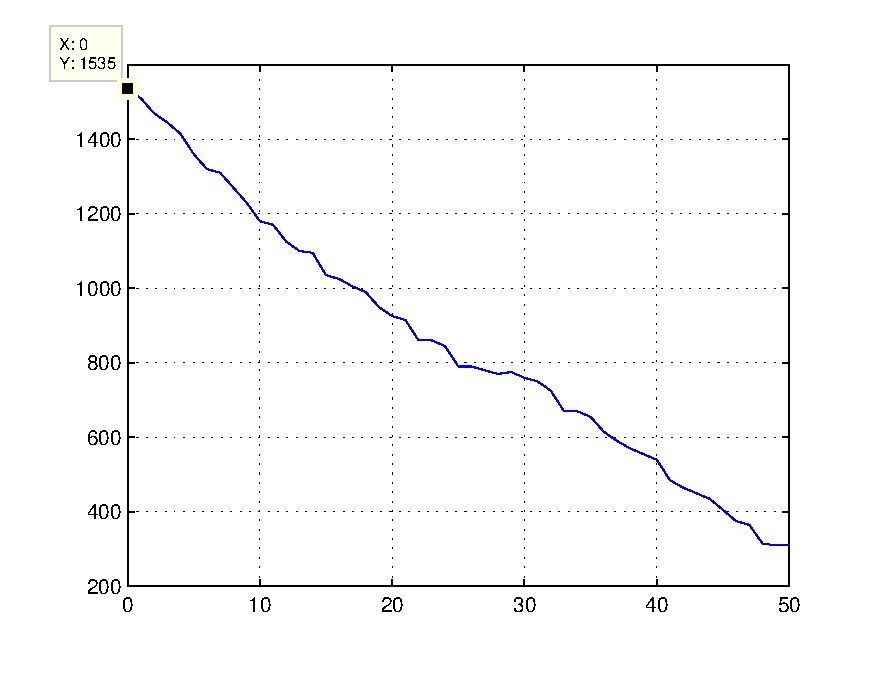
\includegraphics[width=0.4\textwidth]{grafika/probna/Forward/L=0}
	}
	\subfigure[L=10: l1=30, l2=30, l3=40, l4=0]{
	  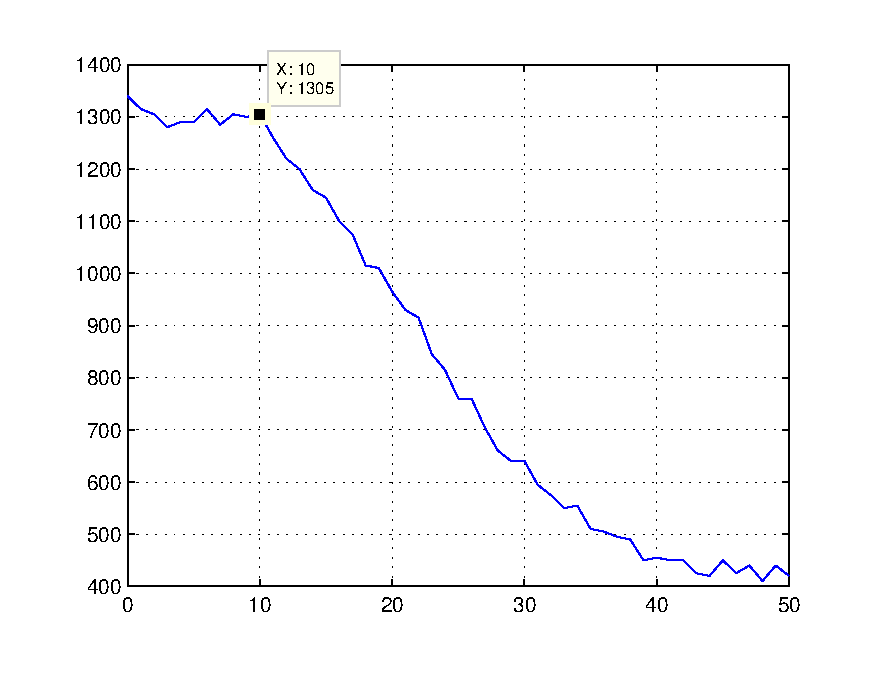
\includegraphics[width=0.4\textwidth]{grafika/probna/Forward/L=10}
	} \\
	\subfigure[L=20: l1=20, l2=40, l3=40, l4=0]{
	  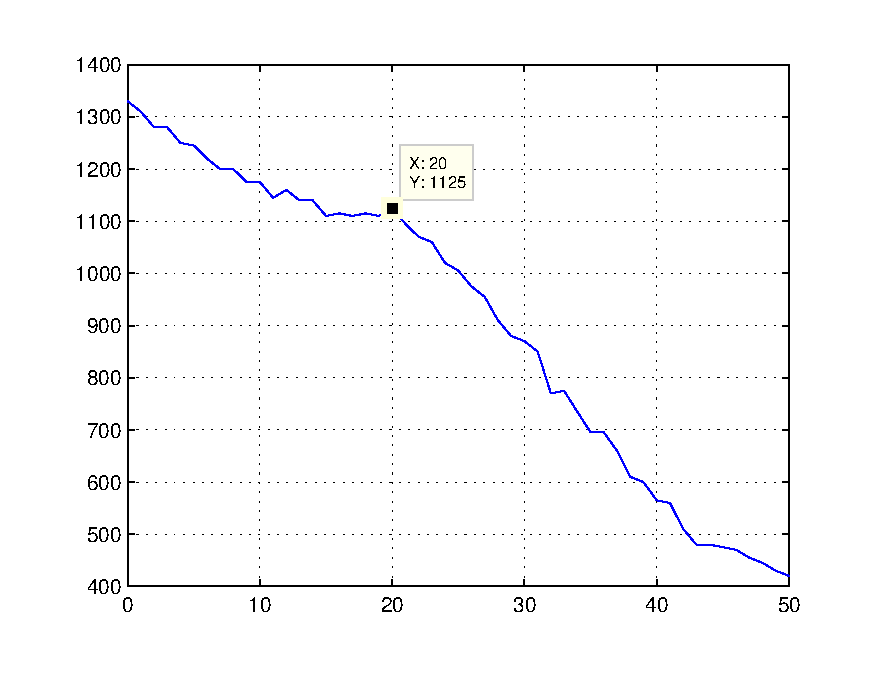
\includegraphics[width=0.4\textwidth]{grafika/probna/Forward/L=20}
	}
	\subfigure[L=30: l1=20, l2=30, l3=50, l4=0]{
	  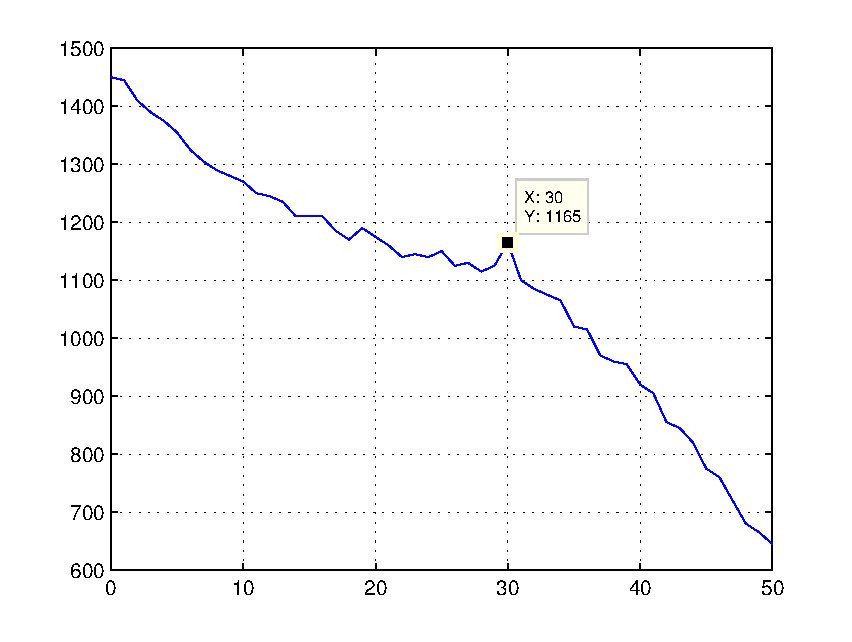
\includegraphics[width=0.4\textwidth]{grafika/probna/Forward/L=30}
	} \\
	\subfigure[L=40: l1=20, l2=30, l3=50, l4=0]{
	  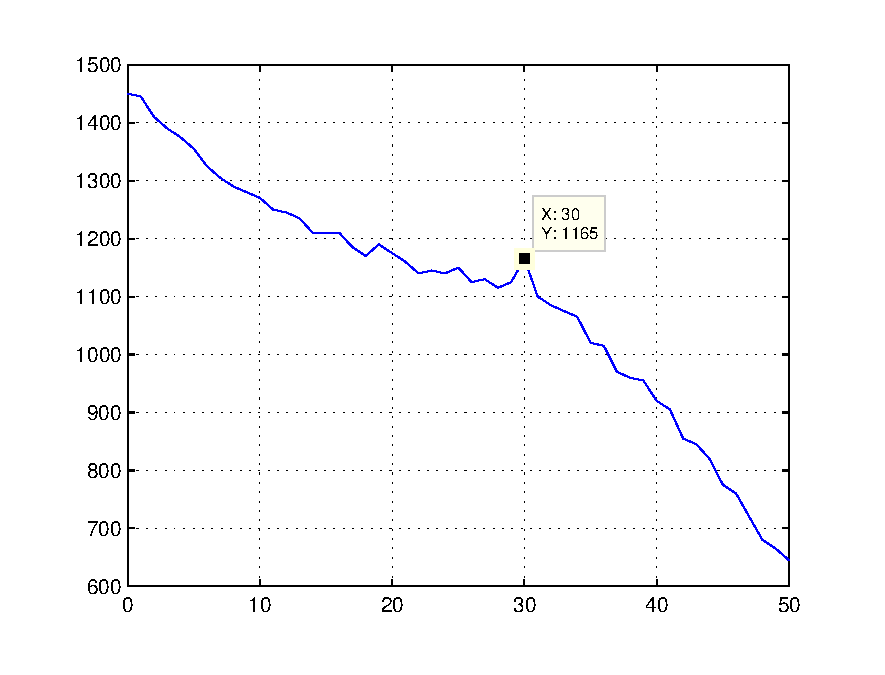
\includegraphics[width=0.4\textwidth]{grafika/probna/Forward/L=40}
	}
  \label{rys:probna_wersja_prosta_kin}  
  \caption{Powierzchnia przestrzeni roboczej w zależności od odległości początków pierwszych ramion 
  manipulatora przy wykorzystaniu prostej kinematyki}

\end{figure}

\begin{figure}[tp]
  \setlength{\unitlength}{1.0cm}
  \centering
	\subfigure[L=0: l1=30, l2=40, l3=30, l4=0]{
	  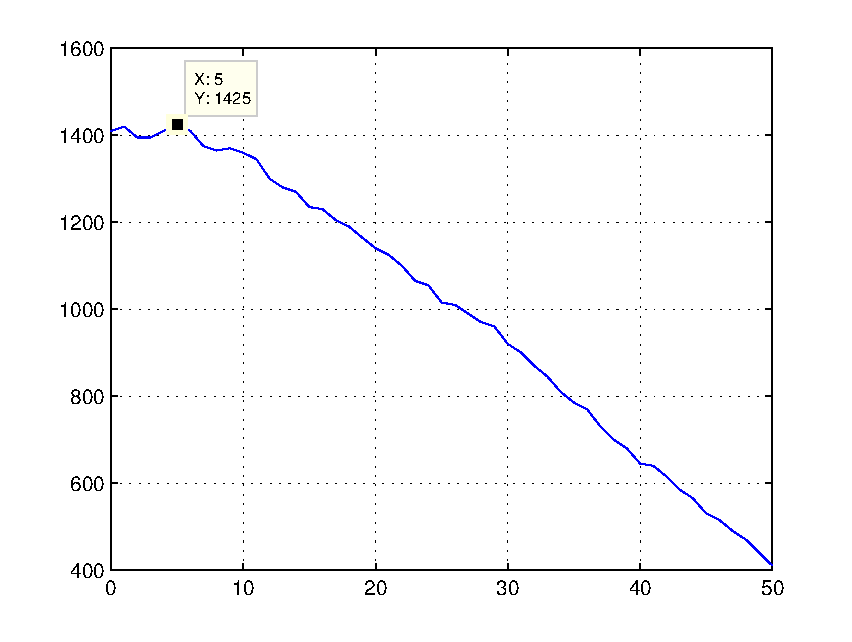
\includegraphics[width=0.4\textwidth]{grafika/probna/Inverse/L=0_inv}
	}
	\subfigure[L=10: l1=30, l2=40, l3=30, l4=0]{
	  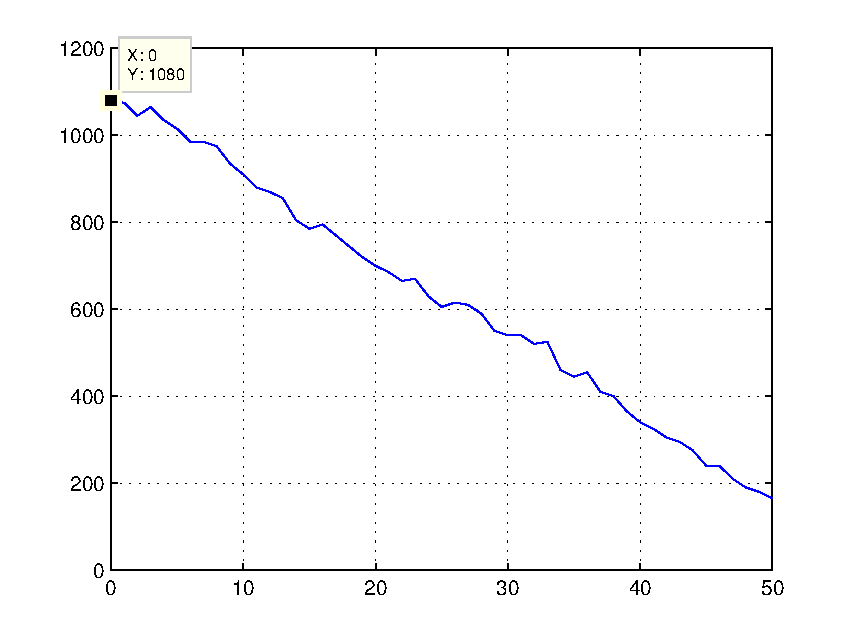
\includegraphics[width=0.4\textwidth]{grafika/probna/Inverse/L=10_inv}
	} \\
	\subfigure[L=20: l1=30, l2=30, l3=40, l4=0]{
	  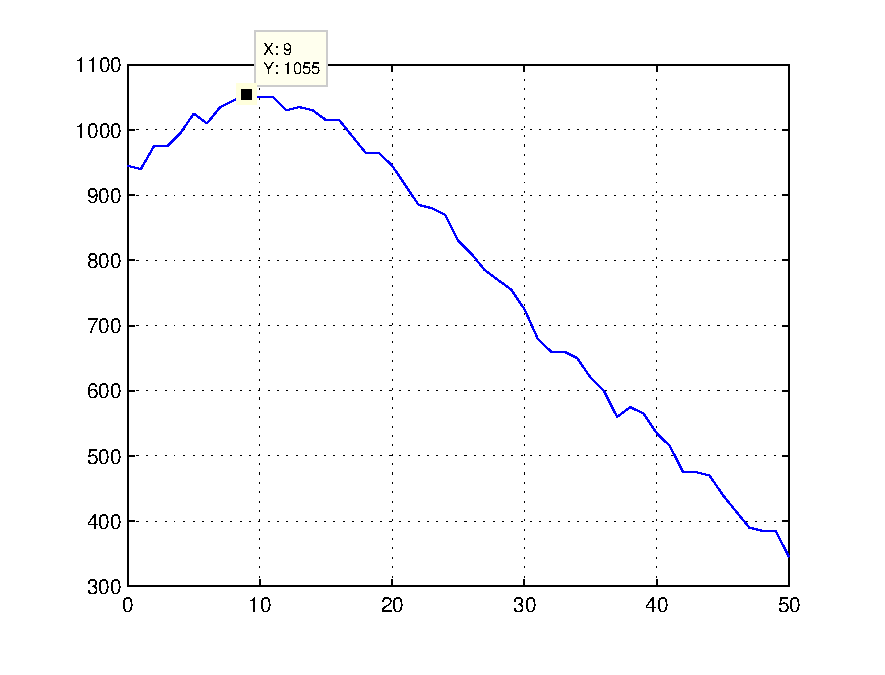
\includegraphics[width=0.4\textwidth]{grafika/probna/Inverse/L=20_inv}
	}
	\subfigure[L=30: l1=30, l2=20, l3=50, l4=0]{
	  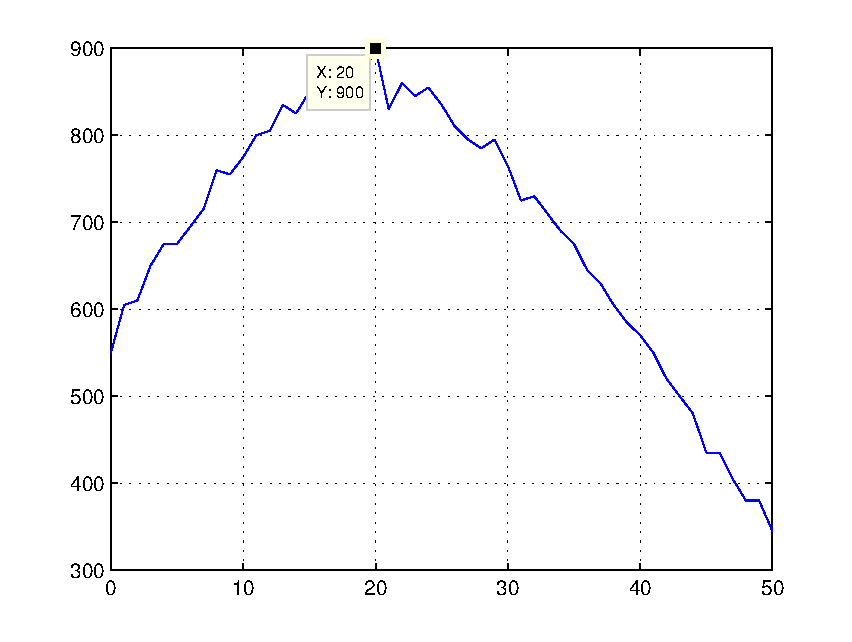
\includegraphics[width=0.4\textwidth]{grafika/probna/Inverse/L=30_inv}
	} \\
	\subfigure[L=40: l1=20, l2=30, l3=50, l4=0]{
	  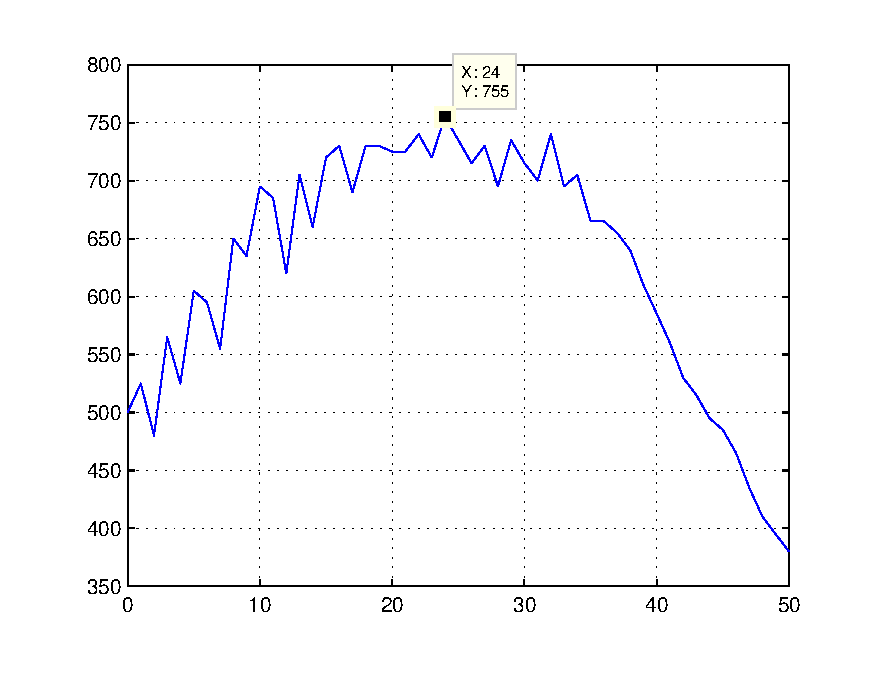
\includegraphics[width=0.4\textwidth]{grafika/probna/Inverse/L=40_inv}
	}
  \label{rys:probna_wersja_odwrotna_kin}  
  \caption{Powierzchnia przestrzeni roboczej w zależności od odległości początków pierwszych ramion 
  manipulatora przy wykorzystaniu odwrotnej}

\end{figure}

\subsection{Wyznaczenie wymiarów ostatecznej wersji manipulatora}

\chapter{Podsumowanie projektu}



\appendix
\chapter{Zawartość płyty CD}
Do pracy dołączono płytę CD zawierającą:
\begin{enumerate}
\item Aplikacja -- katalog zawierający kod źródłowy aplikacji,
\item Doc -- katalog zawierający dokumentację kodu źródłowego przy wykorzystaniu środowiska Doxygen
\item KDL -- katalog zawierający kod źródłowy biblioteki KDL \cite{KDL}
\item Projekt\_Inzynierski.pdf -- wersja elektroniczna niniejszego dokumentu
\end{enumerate}

\addcontentsline{toc}{chapter}{Bibliografia} %utworzenie w spisie treści pozycji Bibliografia
%bibliografia
\bibliography{bibliografia} % wstawia bibliografię korzystając z pliku bibliografia.bib - dotyczy BibTeXa, jeżeli nie korzystamy z BibTeXa należy użyć otoczenia thebibliography




%opcjonalnie może się tu pojawić spis rysunków i tabel
% \listoffigures
% \listoftables


\end{document}

